\chapter{Machine Learning Background}
\label{cha:ML}

This chapter gives an introduction and explanation of several machine learning techniques and the theory behind them. The areas to be explored include: supervised learning, neural networks, convolutional neural networks, surrogate machine learning models and transfer learning. 
\\

\noindent
For a more detailed explanation of the theory and workings of machine learning, see \cite{bishop2006pattern}.


\section{Supervised Learning} \label{supervised}

In the fields of engineering and science, models are frequently produced in order to simulate mathematical or natural phenomena. In these areas, accurate information regarding the phenomena they study. Such information allows the testing of scientific hypothesis and forecasting of future events. But what defines a model? \\

\noindent 
What is common to almost all models is the presence on input variables  and outputs . The model will use a set of input values (which we'll refer to as x) to calculate an outputs values (which we'll refer to as y) that are of interest to those using them. We can approach the development of such models from a hard computing angle: that is, we can hardcode relationships between inputs and outputs based on known relationships. \\

\noindent
Lets look at an example from the domain we are studying in this PhD thesis. In the  field of nuclear engineering, it is important to be able to calculate the power output of a nuclear reactor (which we'll measure in kilowatts) as a function of conditions within the core (\ref{hard_power}).

\begin{equation} \label{hard_power}
	Power(kW)  \rightarrow f\{x\}
\end{equation}

\noindent
In this example, an output value (power) is calculated as a function of input variables (x). There are of course a multitude of other factors that affect core power, however, the point of this example can be made with these four:

\begin{enumerate}
	
	\item \textbf{Fuel Enrichment:} The useable content of the nuclear fuel at the time fuel is inserted into the core. Power level would increase linearly as enrichment rises. This value is measured as a percent of the total mass of the fuel and is usually between 1\% and 5\%.
	 
	\item \textbf{Time Since Refuelling:} The length of time since the core was refuelled. As this time increases, the power level would tend to drop as the useable content of the fuel is used up. This power fall would be linear at first, but the rate would accelerate  after a certain point due to the build up of fission poisons within the core. This value is measured in hours.
	
	\item  \textbf{Flowrate of Coolant:} The rate at which coolant is pumped into the core. This has a positive correlation with core power at lower rates, as the coolant (usually water) helps to sustain the nuclear chain reaction. However, this relationship breaks down after a certain flowrate, as certain concentrations of water act to block the fission sustaining neutrons. The flowrate would  is measured in $m^3$ per second.
	
	\item \textbf{Insertion Depth of Control Rods:} The control rods are inserted in order to slow or halt the nuclear chain reaction. Therefore, there is a negative correlation between insertion depth and power level. Lowering the power through control rod insertion has knock on effects, so the relationship is closer to the reciprocal of the square of the insertion depth.
\end{enumerate}

\noindent
Using the relationships between these inputs at the output we wish to calculate, it would be possible to formulate a model to calculate reactor power output as a function of core configuration. However, from the complex relationships we discuss above, this would not be a trivial undertaking. The production of an effective model through hard computing techniques would require a strong understanding of the physical phenomena underpinning each factor. It would also be intensive in terms of effort from human domain experts. \\

\noindent
Alternatively, a model of this phenomena can be produced using soft computing techniques \cite{ibrahim2016overview} such as machine learning. Rather than hard coding relationships, a stochastic model is produced and optimised using a dataset containing examples of outputs and corresponding inputs. \\

\noindent
In machine learning terms, the output of the model discussed above can be calculated in the form of (\ref{soft_power}) .

\begin{equation} \label{soft_power}
	Power(kW)  \rightarrow f\{x, w, b\}
\end{equation}

\noindent
In this form, the output value of reactor power is calculated as a function of of our core configuration inputs (x) and a weight vector and a scalar bias factor. In machine learning practice, the input variables are referred to as features and the outputs are referred to as predictions. In our above example, there are four features (M = 4). \\

\noindent
The predictions of the model are generated on an instance by instance basis i.e. there is one predicted output per core configuration. The predicted output, which we will refer to as $\hat{y}$, is calculated for a for a given instance, i, in the form of (\ref{instance_prediction}).

\begin{equation} \label{instance_prediction}
	\hat{y}_i = x_i \space \cdot \space w + b
\end{equation}

\noindent 
In (\ref{instance_prediction}), the instance feature vector, defined as $x_i$, is simply the input values for the instance. The dot product between the instance feature vector and the weights vector, w, is calculated and then summed with the bias scalar.  For simplicity, we generally include the bias term when discussing the weights and to that end we shall define an extended weights vector which includes w and b (\ref{expanded_w}).

\begin{equation} \label{expanded_w}
	wb^T = [w_1, w_2 ... w_M, b]
\end{equation}

\noindent
At the start of machine learning model development, the expanded weights vector is initialised with random starting values. The values are then optimised through a model training process. To do this, we need a dataset including multiple instances of reactor power at various configurations of the core. For each instance in our dataset, there will be an input value for each of our features ($x_i$) as well as a corresponding output value that we refer to as the label (y). We refer to these input/output pairs as ground truth values - they are the base data that the model learns and evaluates its optimisation against.
\\

\noindent
The ultimate goal is to optimise the values of wb so that (\ref{instance_prediction}) can be used to make predictions ($\hat{y}_i$) that accurately reflect the ground truth labels ($y_i$). To make this optimisation, we must use a process known as gradient descent \cite{ruder2016overview} where values of wb are updated iteratively based on the derivative of difference between the predictions and ground truth. \\

\noindent
In order to perform the gradient descent operation and to evaluate the performance of our machine learning model, we require a loss function \cite{wang2022comprehensive}. This is a metric used to calculate the difference between the predictions of the model and the ground truth labels. Various ways exist to calculate the loss function, each having their own advantages and applications. Perhaps the simplest form the loss function can take is the mean absolute error \cite{willmott2005advantages}.\\

\begin{equation} \label{mae}
	\lambda_{mae} = \frac{1}{n}\sum_{i=1}^n | y_i - \hat{y_i} | 
\end{equation}

\noindent
Using (\ref{mae}), we can calculate a direct measure of the performance of the model against the ground truth, with the lower the value of $\lambda$, the better the model is performing.  We can also calculate the derivative of the loss function with regards to each element of the vector wb i.e. we can determine how much the loss function changes with a change in each weight. \\

\begin{equation} \label{derivative}
	{\Delta_{wb}}^T = [\frac{\delta\lambda}{\delta w_1}, \frac{\delta\lambda}{\delta w_2} ... \frac{\delta\lambda}{\delta w_M}, \frac{\delta\lambda}{\delta b}]
\end{equation}

\noindent
This derivative (\ref{derivative}) can be used to adjust the extended weights vector, wb, to a set of more more optimal values. This is done by multiplying the derivative, $\Delta_{wb}$, by the user defined scalar value $\alpha$, which is referred to as the learning rate. The values of this vector is then subtracted element-wise from the expanded weights vector to produce a new vector which can then be used again to make instance predictions as per (\ref{instance_prediction}). \\
 
 \begin{equation} \label{gradient_descent}
 	wb_{updated} = wb - (\alpha \cdot \Delta_{wb})
 \end{equation}
 
 \noindent
As can be seen from (\ref{mae}) the loss function (and its derivative) is an average over a set number of instances, n. Lets say the training process has access to a dataset of size N. We can perform the calculation from (\ref{gradient_descent})  using the entire dataset (n = N), a sample batch of the dataset (n $\subset N$), or a single instance (n = 1). If using a single instance or batch to update the weights (known as stochastic gradient descent \cite{ketkar2017stochastic}), the rest of the training set will be iteratively used to perform the same updating calculation. After updating using all instances in the dataset, it is unlikely that the expanded weights vector will be of the most optimal values.  Therefore, this process will be repeated a number of cycles known as epochs.

\begin{figure*}[h]
	\centering
	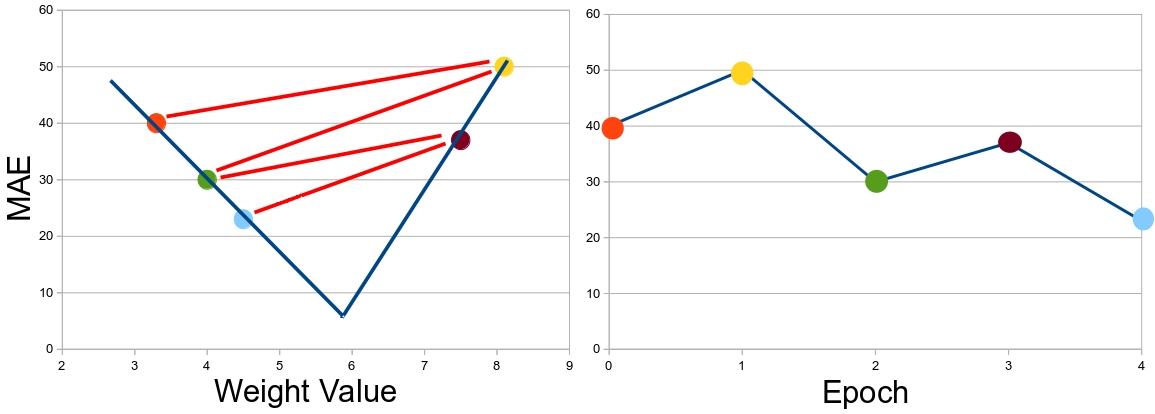
\includegraphics[scale=0.35]{Figures/gradientDescent_mae_bigLR.jpg}
	\caption{Machine Learning Model Training Process (Example 1)} {In this example, a machine learning model is trained over a period of four epochs. The mean absolute error (MAE) loss function is used as well as a relatively large learning rate which reduces each epoch (decay). \textbf{Left}: Loss history against the value of a single model weight.  \textbf{Right}: Loss history against epoch number.}
	\label{fig:GD_maeBigLR}
\end{figure*}

\noindent
In Figure~\ref{fig:GD_maeBigLR}, we see a representation of the training of a machine learning model. We see the progressive loss function calculated over a four epoch interval. This is expressed in two ways: (1) against the value of one of the model weights and (2) against the epoch number.  In this training example, gradient descent is performed using the MAE loss function and a relatively high loss function. This example also shows learning rate decay \cite{lewkowycz2021decay}, where the learning rate is reduced by 10\% successively after each epoch. \\

\noindent 
As mentioned previously, in most machine learning models, there will be multiple weights to optimise (one for each input feature). However, for this illustrative example, we will just focus on the optimisation of one weight.\\

\noindent
The chart on the left of Figure~\ref{fig:GD_maeBigLR} shows a theoretical topology of loss as a function of the example weight (dark blue lines at approximately 45 degrees from one another). At the start of training, we don't know the shape or nature of this topology, it is revealed through the training process. The target for any machine learning training operation is optimise all weight values to produce a model capable of achieving the lowest possible loss value - in the case of Figure~\ref{fig:GD_maeBigLR}, that is the hinge-point between the two dark blue lines. \\

\noindent 
In the aforementioned example, we can see that at the start of training (epoch 0), the weight is initialised at a value of around 3.2 which results in a MAE of about 40. From the gradient of the dark blue line at this point, it can be seen that increasing the weight of the value will tend to reduce the MAE. Feeding this negative gradient and the high learning rate into the subtractive term of (\ref{gradient_descent}) , we get an increased value of our example weight. As can be seen from the the loss time history, this operation actually results in an overshoot leading to a MAE that's actually higher than it was at the start of training (it now has a value of 50). This undesirable outcome is associated with a learning rate which is too high. \\

\noindent
For epoch 2, this time we are at a point in the loss-weight value topology where MAE is tending to increase as the weight value increases: a positive  . Recall that in this example, a learning rate decay is applied, meaning that the learning rate is 10\% lower than it was in the first epoch. This in turn means that the magnitude of the subtractive right-hand-side term of (\ref{gradient_descent}) is 10\% lower than it was in epoch 1. This reduction means that the updated weight is updated to a slightly higher point than the initialisation value. \\

\noindent
The following two epochs follow the same trend, however, the decaying loss rate means that progress towards the MAE minima slows. Further training would eventually see convergence with the weight and corresponding MAE value oscillating around a central value. At this point, further training is off little practical benefit. The practitioner may be able to manually apply early stopping \cite{yao2007early} or experimentally increase the number of epochs until this convergence point is reached. \\ 

\noindent
If we did not apply learning rate decay with the model training configuration of the aforementioned example , we may see a situation where a training process where the model fails to make any progress and repeatedly oscillates between the same two points. \\

\noindent
Lets now look at another example of gradient descent with alternative parameters. In our first example, we used the mean absolute error (MAE) loss function, now we will use instead the mean squared error (MSE) loss function (\ref{mse}). \\

\begin{equation} \label{mse}
	\lambda_{mse} = \frac{1}{n}\sum_{i=1}^n (y_i - \hat{y_i})^2
\end{equation}

\noindent
The mathematical difference between the MAE and MSE loss functions is that the inner term (the difference between the model prediction and ground truth label) is squared rather than simply the absolute. This alternative loss function has two practical differences in model training: 

\begin{enumerate}
	\item  Ground truth labels which are particularly large impact the loss calculation more severely. This can be beneficial when accurate prediction of outliers is of high importance.
	
	\item The loss-weight value topology is a curved U-shaped bend, rather than straight lines at a sharp angle (dark blue in the left of Figure~\ref{fig:GD_mseSmallLR}). This is because the derivative of this function with regards to the residual ($y_i - \hat{y_i}$) is variable rather than constant.
\end{enumerate}

\noindent
The other change is that we will assume a smaller initial learning rate than in the previous example.  In addition, we will not be decaying the learning rate. We begin with the same weight initialisation as the first example and loss starting point\footnote{In practice, the same residual ($y_i - \hat{y_i}$) would result is a different loss value for MAE and MSE (after all, they are different functions), but for these examples we assume equivalent values are calculated for each.}. \\

\begin{figure*}[h]
	\centering
	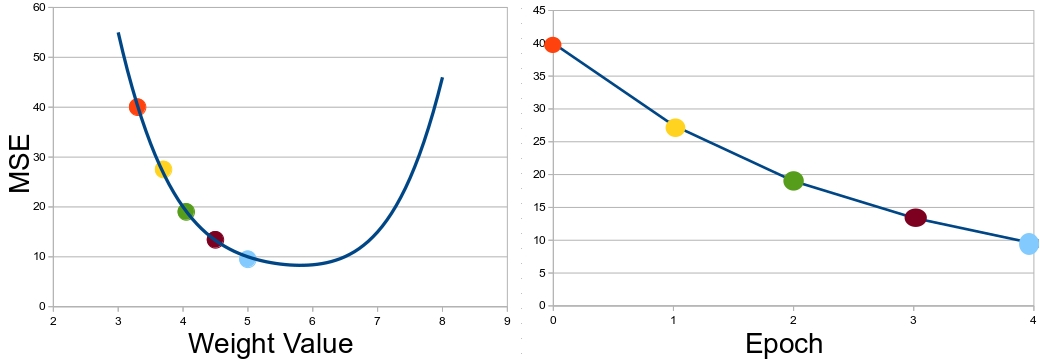
\includegraphics[scale=0.35]{Figures/gradientDescent_mse_smallLR.jpg}
	\caption{Machine Learning Model Training Process (Example 2)} {In this example, a machine learning model is trained over a period of four epochs. The mean squared error (MSE) loss function is used as well as a relatively small learning rate. \textbf{Left}: Loss history against the value of a single model weight.  \textbf{Right}: Loss history against epoch number.}
	\label{fig:GD_mseSmallLR}
\end{figure*}

\noindent
From Figure~\ref{fig:GD_mseSmallLR}, it can be seen that after one epoch of training, the weight value is updated only a small amount on account of the smaller learning rate. At this new point, the gradient of loss with regards to weight value is still negative, albeit to a smaller magnitude. On account of the subtractive term of (\ref{gradient_descent}) being smaller, the weight value update for the second epoch is somewhat smaller than the first. This trend can be seen to continue towards the base of the base of the curve. \\

\noindent
Comparing the performance of the two model training processes, it is possible to see the apparent advantages of the second configuration.  However, in practice different parameters have application in varying circumstances and conditions. The exact combination of parameters that are optimal for each problem must be determined through precedent (techniques found to be effective in previous works) and through experimentation.  \\

\noindent
In the previous examples, we saw the gradient descent method used to minimise loss towards the nadir of a loss topology. However, the topology for the full problem space might contain multiple minima regions. 

\begin{figure*}[h]
	\centering
	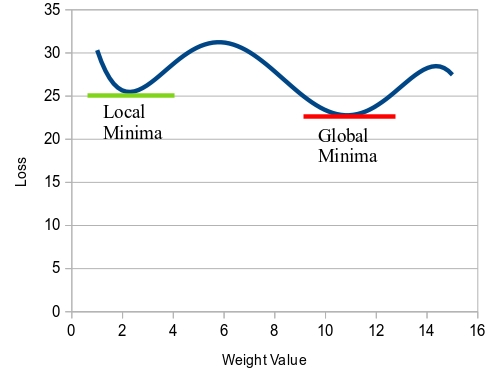
\includegraphics[scale=0.45]{Figures/loss_minima_maxima.jpg}
	\caption{Global Topology of Loss as a Function of Weight Value} {When looking at the full topology for the entire problem space, we see that there are there may be more than a single minima. }
	\label{fig:minima_maxima}
\end{figure*}
		
% Training set, testing set
% At the end of training, we use testing set to evaluate.		
		
% Local minima - how to overcome? 
		% Repeating experiments
		% Loss rate - too high, too low, dynamic
		% optimiser
		
% Another problem is that a machine learning model in this format can only model linear relationships between input variables and outputs. Therefore, this method may not be optimal for modelling the example scenario above as there is a complex relationship between some inputs and the output value. For example, increasing the flowrate acts to increase and then decrease the power at different levels. To produce a machine learning model capable of accounting for these non-linear complexities, we must look to neural networks.		
 		

\section{Neural Networks} \label{NN}

Neural networks can be seen as a multi-layer stacking of the type of operation described in section~\ref{supervised}. The point at which each of these operations occurs is usually referred to as a neuron or node. Neurons are placed in parallel or sequence (Figure~\ref{fig:neural_network}) to form the model architecture. Various arrangements of these nodes may be employed, with varying depth and width of the network. 
\\

\noindent
Differing neural network architectures with varying hyper-parameters \cite{gurney1997introduction} can be employed in the design of a machine learning model. The architecture of a neural network consists of nodes at which a mathematical operation is performed. The nodal output is passed through an activation function which transforms it in a non-linear manner. Commonly employed activation functions include the rectified linear unit (ReLu) \cite{hara2015analysis} and the Softplus function \cite{zheng2015improving}. 
\\

\noindent
The design of a neural network usually features multiple cascading layers, with the output of the previous layer feeding through as input to the subsequent layer. The network is trained through application of the back-propagation algorithm \cite{hecht1992theory} which uses the loss function to adjust the weights throughout the network. The back-propagation algorithm utilises a learning rate, a user defined value that determines how quickly the model weights are adjusted. A learning rate value must be chosen so as not be too high or low: either extreme will prevent an optimal solution from being attained. The learning rate may be adjusted during training. 
\\

\noindent
At the start of neural network training - prior to the back-propagation process - the trainable parameters of the model are initialised with random values. Repeating the initialisation and training process several times, a different set of optimised weights will be produced each time, despite using the same training data. To account for this stochastic nature of the training process, machine learning experiments are normally repeated several times.
\\

\noindent
A common problem encountered during the training of neural networks is that of overfitting \cite{hawkins2004problem}. This phenomenon is encountered when a model fits so closely to a training dataset that it does not perform well on new data that it has not encountered during training i.e. the model does not generalise well. A significantly lower training loss relative to the test loss indicates overfitting, whereas a similar value for the two loss values indicates good general performance of the model. To avoid overfitting, several regularisation techniques are employed. These include adding a term to loss function that penalises large weights and randomised dropout of model layers \cite{srivastava2014dropout}. 
\\

\noindent
Several configurations of neural networks are available. A common choice is the fully connected or dense neural network (DNN): i.e. the output of every node in a layer feeds into every node in the subsequent layer, leading to a 'dense' architecture. An alternative configuration is the convolutional neural network (CNN) discussed in the following chapter. 

\begin{figure*}[p]
	\centering
	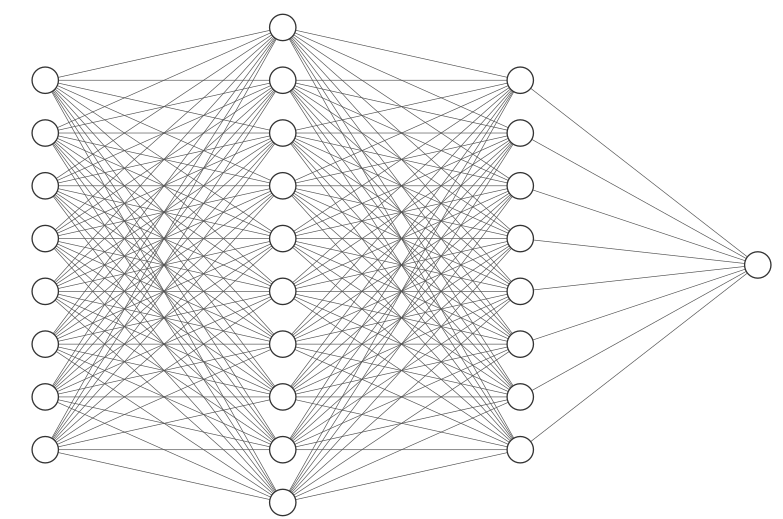
\includegraphics[scale=0.6]{Figures/nn.png}
	\caption{Neural Network: An example of a feed-forward network.} {From left to right: input layer accepting 8 features; first 'hidden' layer with 10 nodes, each fully connected to every node in the previous layer; second 'hidden' layer this time with only 8 nodes, again is fully connected to accept the output of each node from the previous layer; a single output node which is fully connected to each node from the previous layer.}
	\label{fig:neural_network}
\end{figure*}

\begin{figure*}[p]
	\centering
	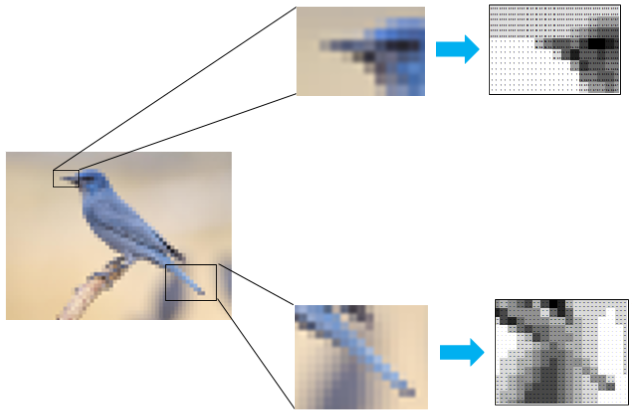
\includegraphics[scale=0.75]{Figures/cnn_feature.png}
	\caption{Convolutional Neural Network: Feature Extraction.}
	\label{fig:cnn_feature}
\end{figure*}

\section{Convolutional Neural Networks (CNN)} \label{convolution}

Convolutional neural networks (CNNs) attempt to capture local signals in data by use of a sliding window which passes over the input space. CNNs have been utilised in several areas of image analysis, including cell detection in medicine \cite{xie2015beyond} and depth estimation in photographs \cite{li2015depth}. Within the engineering field, they have been employed to predict remaining useful life of components \cite{babu2016deep}. The application of CNNs may be effective in the research problem discussed in this thesis as there are similarities between the data format for AGR graphite core analysis and image recognition, with the presence and identification of local arrangements important in both areas.
\\

\begin{figure*}[p]
	\centering
	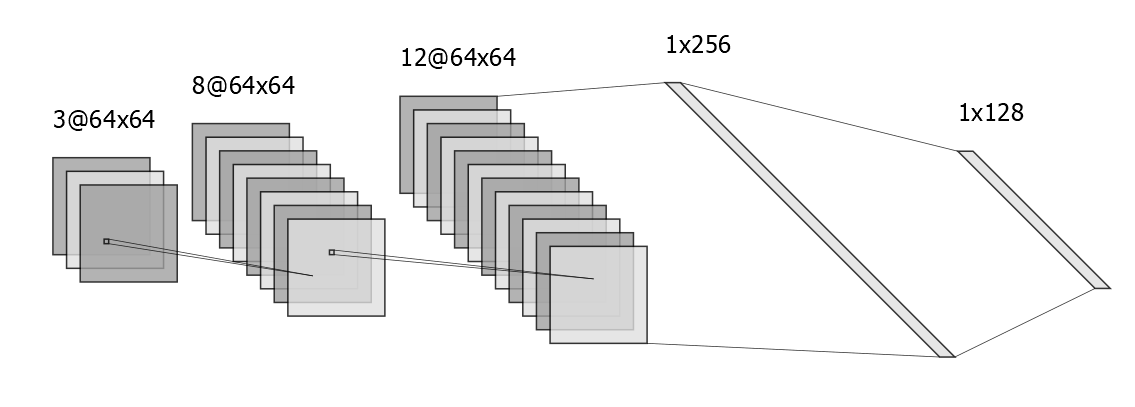
\includegraphics[scale=0.45]{Figures/cnn_arch.png}
	\caption{Convolutional Neural Network: Architecture.}
	\label{fig:cnn}
\end{figure*}

\section{Surrogate Machine Learning Models} \label{Surrogate}

For any given natural phenomena, it is possible to develop a physical model that mathematically describes it and can approximate its behaviour. Such phenomena range from a simple decaying wave (Figure~\ref{fig:surrogate}) to highly complex models such as that of turbulent fluid movement. Such models are unlikely to ever be a perfect representation of the natural phenomena, as there may be too many variables and factors to ever account for them all, hence there will always be some disparity. However, it may be possible to produce a model that is accurate enough so as to provide data that is of practical use.
\\

\noindent
From  data generated by such mathematical models, it is possible to train machine learning models to produce equivalent outputs from the same inputs. This will effectively be an additional layer of approximation on top of an already approximate model.
\\

\noindent
What is the motivation for doing this? Given a mathematical model of a phenomena, why develop and use a surrogate model using machine learning which provides inferior results? It is difficult to see why given the simple example of Figure~\ref{fig:surrogate}. However, in a real world case, such as nuclear reactor core safety, such a model may be highly complex, involving thousands of parameters and requiring significant computational expense. A machine learning model on the other hand, once trained, is computationally cheap to use, being just a series of matrix operations. The production of such a machine learning surrogate can also be seen as an exploration of the data space i.e. it is likely through the process of model training and refinement that insights into relationships between variables will be discovered. It may also be possible to develop machine learning tools so as to work in symbiosis with traditional mathematical models, with one informing the direction and focus of the other.
\\

\begin{figure*}[p]
	\centering
	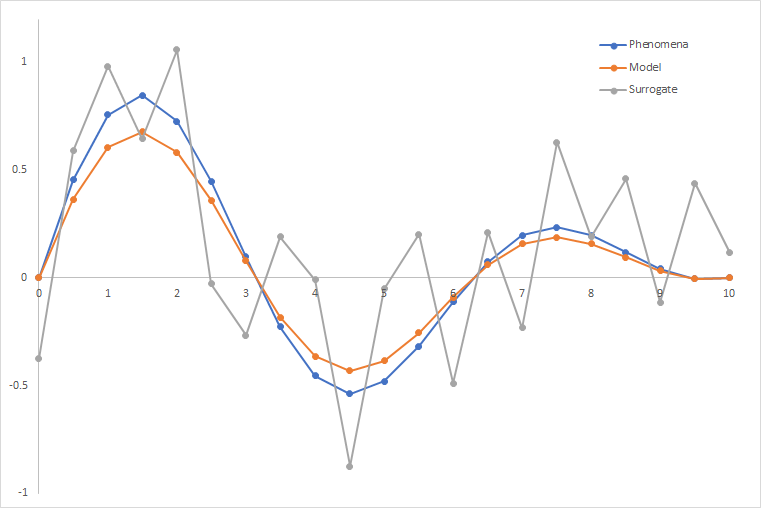
\includegraphics[scale=0.65]{Figures/surrogate_model.png}
	\caption{Modelling of Natural Phenomena} {A decaying wave (blue). A mathematical model may be developed which approximates its behaviour (orange). It may be possible to build a surrogate model (grey) which is an approximation built upon an approximation.}
	\label{fig:surrogate}
\end{figure*}

\begin{figure*}[h]
	\centering
	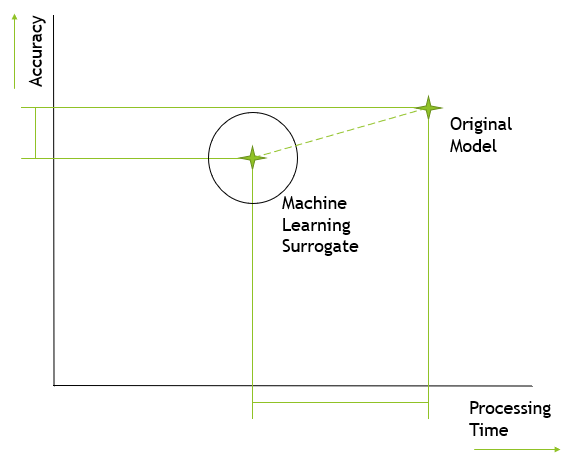
\includegraphics[scale=0.65]{Figures/MLS_vs_OM.png}
	\caption{The Trade-off Between a Machine Learning Surrogate Model and the Original Model} {Once trained on data from the original model, the production of new data is likely to be significantly more efficient in terms of computation and time. However, as the machine learning model is produced using data from the original model, there will be some inevitable reduction in accuracy.}
	\label{fig:surrogate_vs_model}
\end{figure*}

\noindent With each layer of approximation, there is of course an added margin of inaccuracy. Therefore, the development of a machine learning surrogate model is a trade-off between computational expense/time and accuracy (Figure~\ref{fig:surrogate_vs_model}).

\section{Transfer Learning and Existing ML Models} \label{transfer}

Many organisations have produced highly optimised neural networks, often demonstrating their capabilities in public competitions such as ImageNet \cite{russakovsky2015imagenet}. The successful competitors often publish their model architectures along with the best performing weights. Models produced and published through this competition include VGG \cite{simonyan2014very} and ResNet \cite{he2015deep}. Although these models are optimised to perform image classification tasks, many researchers have found that the aforementioned models can be adapted to other areas of study in a process known as transfer learning \cite{tan2018survey}.

\section{Relevant Literature}

An overview of machine learning techniques and their application to nuclear engineering is given in a recent paper \cite{gomez2020status}. This review details a range of machine learning approaches, including decision trees, nearest-neighbour, support vector machines, naive bayes, as well as Convolutional and recurrent neural networks. It then goes on to outline how these techniques have been applied in nuclear engineering fields such as plant health, radiation protection and optimisation. Although this paper does not reference the AGR or graphite, it does provide a useful introduction to the field. 
\\

\noindent
The same authors produced an earlier paper in which they use a neural network to predict the response of a light water reactor to various operational and accident conditions \cite{fernandez2017nuclear}. The motivations for this work include an ability to make rapid safety decisions (i.e. greater computational efficiency) as well as providing insight into safety issues. This research highlights various neural network architectures as shown in Figure~\ref{fig:architectures}.  
\\

\begin{figure*}[p]
	\centering
	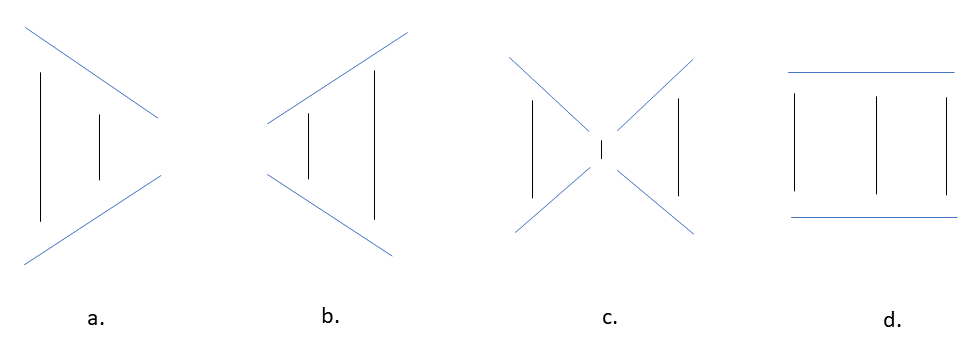
\includegraphics[scale=0.5]{Figures/architecture.png}
	\caption{Four Possible Neural Network Architectures} {Input on the left, output on the right. \textbf{(a)}: a narrowing structure where layers decrease in size towards the output layer and the output vector is smaller than the input vector; \textbf{(b)}: the inverse of a. with the layers increasing in size towards the output layer; \textbf{(c)}: An architecture combining both of the previous approaches, with the structure compressing the input and then expanding it before the output layer; \textbf{(d)}: A parallel structure where the layers remain of roughly similar size across the network. This Figure is a reproduction of Fig. 4 from \cite{fernandez2017nuclear}.}
	\label{fig:architectures}
\end{figure*}

\noindent
Academic works which apply machine learning to the production of engineering surrogates can be found as far back as 2003, where \cite{javadi2003neural} developed a symbiotic approach combine finite element models and neural network architecture. A more recent treatment of this topic can be found in \cite{kim2019machine} where the authors employ several approaches. These include an adaptive sampling method, where instances are generated and included in the training set based on their importance: i.e. selecting samples within the problem space that maximise useful information and excluding those which contain redundancy. Another relevant work is \cite{zeng2018machine} which uses a machine learning model to predict subsequent molten reactor core behaviour based on a time history. To train the ML model used in this work, the researchers generate data using a traditional engineering model (equivalent to that described in section \ref{Engineering}) to build a surrogate model (as described in section \ref{Surrogate}).  
\\

\noindent
A particularly relevant existing work to the PhD project discussed in this thesis is \cite{dihoru2018neural} which concerns both AGR graphite and machine learning. These researchers use data from a physical model of an AGR reactor which simulates an earthquake to train a feed-forward neural network (see Figure~\ref{fig:neural_network}) with 3 layers. The data generated by five configurations of the physical model (one intact, four with random distributions of cracks) are used to generate values for displacement in the top layer of the core. A neural network is then trained on this data, with displacements in the central channel being used to predict displacements in a select number of surrounding channels. The researchers achieve reasonably good agreement between model prediction and the ground truth data from their physical model, although there is some breakdown at the extremes. The scope of this model is somewhat limited, however, in that the model can only predict displacements from displacements at other locations. Superior model performance may also be achieved with a more complex neural network.  
